% -*- TeX-master: "sbml-level-2-version-3"; fill-column: 66 -*-
% $Id$
% $Source$
% ----------------------------------------------------------------

\section{Preliminary definitions and principles}
\label{sec:general}

This section covers certain concepts and constructs that are used
repeatedly in the rest of SBML Level~2.


\subsection{Primitive data types}
\label{sec:primitive-types}

Most primitive types in SBML are taken from the data types defined
in \xmlschemaone~\citep{biron:2000,fallside:2000,thompson:2000}.
A few other primitive types are defined by SBML itself.  What
follows is a summary of the XML Schema types and the definitions
of the SBML-specific types.  Note that while we have tried to
provide accurate and complete summaries of the XML Schema types,
the following should not be taken to be normative definitions of
these types.  Readers should consult the \xmlschemaone
specification for the normative definitions of the XML types used
by SBML.


\subsubsection{Type \primtype{string}}
\label{sec:string}

The \xmlschemaone type \primtype{string} is used to represent
finite-length strings of characters.  The characters permitted to
appear in XML Schema \primtype{string} include all Unicode
characters~\citep{unicode:1996} except for two delimiter
characters, 0xFFFE and 0xFFFF~\citep{biron:2000}.  In addition,
the following quoting rules specified by XML for character
data~\citep{bray:2000} must be obeyed:
\begin{itemize}

\item The ampersand (\texttt{\&}) character must be escaped using
  the entity \texttt{\&amp;}.

\item The apostrophe (\texttt{'}) and quotation mark (\texttt{"})
  characters must be escaped using the entities \texttt{\&apos;}
  and \texttt{\&quot;}, respectively, when those characters are
  used to delimit a string attribute value.

\end{itemize}
Other XML built-in character or entity references, e.g.,
\texttt{\&lt;} and \texttt{\&x1A;}, are permitted in strings.


\subsubsection{Type \primtype{boolean}}
\label{sec:boolean}

The \xmlschemaone type \primtype{boolean} is used as the data type
for SBML object attributes that represent binary true/false values.
\xmlschemaone defines the possible literal values of
\primtype{boolean} as the following: \val{true}, \val{false},
\val{1}, and \val{0}.  The value \val{1} maps to \val{true} and
the value \val{0} maps to \val{false}.

\begin{blockChanged}

Note that there is a discrepancy between the value spaces of type
\primtype{boolean} as defined by \xmlschemaone and \mathml: the
latter uses only \val{true} and \val{false} to represent boolean
values and \val{0} and \val{1} are interpreted as numbers.
Software tools should take care to not to use \val{0} and \val{1}
as boolean values in \mathml expressions.  See further discussion
in Section~\ref{sec:handling-booleans}.

\end{blockChanged}


\subsubsection{Type \primtype{int}}
\label{sec:integer}

The \xmlschemaone type \primtype{int} is used to represent decimal
integer numbers in SBML.  The literal representation of an
\primtype{int} is a finite-length sequence of decimal digit
characters with an optional leading sign (\val{+} or \val{-}).  If
the sign is omitted, \val{+} is assumed.  The value space of
\primtype{int} is the same as a standard 32-bit signed integer in
programming languages such as C, \ie 2147483647 to $-2147483648$.


\subsubsection{Type \primtype{positiveInteger}}
\label{sec:positiveinteger}

The \xmlschemaone type \primtype{positiveInteger} is used to
represent nonzero, nonnegative, decimal integers: \ie 1, 2, 3,
\ldots.  The literal representation of an integer is a
finite-length sequence of decimal digit characters, optionally
preceded by a positive sign (``\token{+}'').  There is no
restriction on the absolute size of \primtype{positiveInteger}
values in XML Schema; however, the only situations where this type
is used in SBML involve very low-numbered integers.  Consequently,
applications may safely treat \primtype{positiveInteger} as
unsigned 32-bit integers.


\subsubsection{Type \primtype{double}}
\label{sec:double}

The \xmlschemaone type \primtype{double} is the data type of
floating point \changed{numerical quantities in SBML}.  It is restricted to IEEE
double-precision 64-bit floating point type IEEE 754-1985.  The
value space of \primtype{double} consists of (a) the numerical
values $m \times 2^x$, where $m$ is an integer whose absolute
value is less than $2^{53}$, and $x$ is an integer between -1075
and 970, inclusive, (b) the special value positive infinity
(\token{INF}), (c) the special value negative infinity
(\token{-INF}), and (d) the special value not-a-number
(\token{NaN}).  The order relation on the values is the following:
$x < y$ if and only if $y - x$ is positive for values of $x$ and
$y$ in the value space of \primtype{double}.  Positive infinity is
greater than all other values other than \token{NaN}.  \token{NaN}
is equal to itself but is neither greater nor less than any other
value in the value space.  (Software implementors should consult
the \xmlschemaone definition of \primtype{double} for additional
details about equality and relationships to IEEE 754-1985.)

\changed{The general form of \primtype{double} numbers is
  \val{$x$e$y$}, where $x$ is a decimal number (the mantissa),
  \val{e} is a separator} \changed{character, and $y$ is an
  exponent; the meaning of this is ``$x$ multiplied by 10 raised
  to the power of $y$'', i.e.,} \changed{$x \times 10^y$.}  More
precisely, a \primtype{double} value consists of a mantissa with
an optional leading sign (\val{+} or \val{-}), optionally followed
by the character \token{E} or \token{e} followed by an integer
(the exponent).  The mantissa must be a decimal number: an integer
optionally followed by a period (\token{.})\ optionally followed
by another integer.  If the leading sign is omitted, \val{+} is
assumed.  An omitted \token{E} or \token{e} and exponent means
that a value of 0 is assumed for the exponent.  If the \token{E}
or \token{e} is present, it must be followed by an integer or an
error results.  The integer acting as an exponent must consist of
a decimal number optionally preceded by a leading sign (\val{+} or
\val{-}).  If the sign is omitted, \val{+} is assumed.  The
following are examples of legal literal \primtype{double} values:
\begin{center}
\begin{tabular}{llllllllllll}
\token{-1E4}, & \token{+4}, & \token{234.234e3}, & \token{6.02E-23}, 
& \token{0.3e+11}, & \token{2}, & \token{0}, & \token{-0}, 
& \token{INF}, & \token{-INF}, & \token{NaN}
\end{tabular}
\end{center}

As described in Section~\ref{sec:formulas}, SBML uses a subset of
the \mathmltwo standard~\citep{w3c:2000b} for expressing
mathematical formulas in XML.  This is done by stipulating that
the MathML language be used whenever a mathematical formula must
be written into an SBML model.  Doing this, however, requires
facing two problems: first, the syntax of numbers in scientific
notation (``e-notation'') is different in MathML from that just
described for \token{double}, and second, the value space of
integers and floating-point numbers in MathML is not defined in
the same way as in \xmlschemaone.  We elaborate on these issues in
Section~\ref{sec:cn-token}; here we summarize the solution taken
in SBML.  First, within MathML, the mantissa and exponent of
numbers in ``e-notation'' format must be separated by one
\texttt{<sep/>} element.  This leads to numbers of the form
\texttt{<cn type="e-notation"> 2 <sep/> -5 </cn>}.  Second, SBML
stipulates that the representation of numbers in MathML
expressions obey the same restrictions on values as defined for
types \primtype{double} and \primtype{int}
(Section~\ref{sec:integer}).


\subsubsection{Type \primtype{ID}}
\label{sec:id}

The \xmlschemaone type \primtype{ID} is identical to the XML 1.0
type \primtype{ID}.  The literal representation of this type
consists of strings of characters restricted as summarized in
Figure~\ref{fig:id}.

% For a good summary of CombiningChar and Extender see
% http://xsd.stylusstudio.com/2003Sep/post05008.htm


\begin{figure}[htb]
  \ttfamily
  \small
  \centering
  \vspace*{-1ex}
  \begin{blockChanged}
    \begin{edtable}{tabular}{lll}
      NCNameChar & ::= & letter | digit | '.' | '-' | '\_' | ':' | CombiningChar | Extender\\
      ID         & ::= & ( letter | '\_' | ':' ) NCNameChar*
    \end{edtable}
  \end{blockChanged}
  \vspace*{-3pt}
  \caption{\changed{Type \primtype{ID}}
    expressed in the variant of BNF used by the XML 1.0
    specification~\protect\citep{bray:2004}.  The characters
    \texttt{(} and \texttt{)} are used for grouping, the character
    \texttt{*} indicates ``zero or more times'', and the character
    \texttt{|} indicates ``or''.  \changed{The production \token{letter}
    consists of the basic upper and lower case alphabetic
    characters of the Latin alphabet along with a large number of
    related characters defined by Unicode~2.0; similarly, the
    production \token{digit} consists of the numerals
    \texttt{0..9} along with related Unicode~2.0 characters.}  The
    \token{CombiningChar} production is a list of characters that
    add such things as accents to the preceding character. (For
    example, the Unicode character \token{\#x030A} when combined
    with `a' produces `\aa'.)  The \token{Extender} production is
    a list of characters that extend the shape of the preceding
    character.  Please consult the XML~1.0
    specification~\protect\citep{bray:2004} for the complete
    definitions of \token{letter}, \token{digit},
    \token{CombiningChar}, and \token{Extender}.}
  \label{fig:id}
\end{figure}

In SBML, type \primtype{ID} is the data type of the \token{metaid}
\changed{attribute} on \SBase, described in
Section~\ref{sec:sbase}.  An important aspect of \primtype{ID} is
the XML requirement that a given value of \primtype{ID} must be
unique throughout an XML document.  All data values of type
\primtype{ID} are considered to reside in a single common global
namespace spanning the entire XML document, regardless of the
\changed{attribute} where type \primtype{ID} is used and
regardless of the level of nesting of the \changed{objects} (or
XML elements).

%In XML, the underlying purpose of using \primtype{ID} is to be
%able to refer to the values using the XML type \primtype{IDREF}.


\subsubsection{Type \primtype{SId}}
\label{sec:sid}

The type \primtype{SId} is the type of the \token{id} \changed{attribute} found
on the majority of SBML components.  \primtype{SId} is a data type
derived from the basic XML type \primtype{string}, but with
restrictions about the characters permitted and the sequences in
which those characters may appear.  The definition is shown in
Figure~\vref{fig:sid}.

\begin{figure}[hbt]
  \ttfamily
  \small
  \centering
  \renewcommand{\arraystretch}{0.9}
  \begin{edtable}{tabular}{lll}
    letter & ::= & 'a'..'z','A'..'Z'\\
    digit  & ::= & '0'..'9'\\
    idChar & ::= & letter | digit | '\_'\\
    SId    & ::= & ( letter | '\_' ) idChar*\\
  \end{edtable}
  \vspace*{-2pt}
  \caption{The definition of the type \primtype{SId}.  (Please see
    the caption of Figure~\protect\ref{fig:id} for an explanation
    of the notation.)}
  \label{fig:sid}
\end{figure}

The equality of \primtype{SId} values is determined by an exact
character sequence match; \ie comparisons of these identifiers
must be performed in a case-sensitive manner.  This applies to all
uses of \token{SId}.

The \primtype{SId} is purposefully not derived from the XML
\primtype{ID} type (Section~\ref{sec:id}).  Using XML's
\primtype{ID} would force all SBML identifiers to exist in a
single global namespace, which would affect not only the form of
local parameter definitions but also future SBML extensions for
supporting model/submodel composition.  Further, the use of the
\primtype{ID} type for SBML identifiers would have limited utility
because \mathmltwo \token{ci} elements are not of the type
\primtype{IDREF} (see Section~\ref{sec:formulas}).  Since the
\primtype{IDREF}/\primtype{ID} linkage cannot be exploited in
MathML constructs, the utility of the XML \primtype{ID} type is
greatly reduced.  \changed{Finally, unlike \primtype{ID},
  \primtype{SId} does not include Unicode character}
\changed{codes; the identifiers are plain text.}


\subsubsection{Type \primtype{UnitSId}}
\label{sec:unitsid}

The type \primtype{UnitSId} is derived from \primtype{SId}
(Section~\ref{sec:sid}) and has identical syntax.  The
\primtype{UnitSId} type is used as the data type for the
identifiers of units (Section~\ref{sec:unitdefinition-structure})
and for references to unit identifiers in SBML objects.
The purpose of having a separate data type for such identifiers is
enable the space of possible unit identifier values to be
separated from the space of all other identifier values in SBML.
The equality of \primtype{UnitSId} values is determined by an
exact character sequence match; \ie comparisons of these
identifiers must be performed in a case-sensitive manner.

\begin{blockChanged}
 
A number of reserved symbols are defined in the space of values of
\primtype{UnitSId}.  These reserved symbols are the list of base
unit names defined in Table~\vref{tab:unitkind}, and the SBML
built-in units \val{substance}, \val{volume}, \val{area},
\val{length}, and \val{time} listed in Table~\vref{tab:builtin}.
These symbols and their use is described in
Section~\ref{sec:unitdefinitions}.

\end{blockChanged}


\subsubsection{Type \primtype{SBOTerm}}
\label{sec:sboterm-type}

The type \primtype{SBOTerm} is used as the data type of
\changed{the attribute \token{sboTerm} on \SBase}.  The type
consists of strings of characters matching the restricted pattern
described in Figure~\ref{fig:sboterm}.

\begin{figure}[htb]
  \ttfamily
  \small
  \begin{blockChanged}
    \begin{center}
      \begin{edtable}{tabular}{lll}
        digit   & ::= & '0'..'9'\\
        SBOTerm & ::= & 'SBO:' digit digit digit digit digit digit digit \\
      \end{edtable}
    \end{center}
  \end{blockChanged}
  \caption{The definition of \primtype{SBOTerm}.  The
    \primtype{SBOTerm} type consists of strings beginning with
    \token{SBO:} and followed by seven decimal digits.  (Please see
    the caption of Figure~\protect\ref{fig:id} for an explanation
    of the notation.)}
  \label{fig:sboterm}
\end{figure}

Examples of valid string values of type \primtype{SBOTerm} are
``\token{SBO:0000014}'' and ``\token{SBO:0003204}''.  These values
are meant to be the identifiers of terms from an ontology whose
vocabulary describes entities and processes in computational
models.  Section~\ref{sec:sboTerm} provides more information about
the ontology and principles for the use of these terms in SBML
models.

% The removal of the previous section 3.2 (diagram of the
% inheritance hierarchy) caused all subsequent section numbers to
% change.  This marks the sections in red to flag the change.

\makeatletter
\renewcommand{\thesection}      {\changed{\@arabic\c@section}}
\renewcommand{\thesubsection}   {\changed{\thesection.\@arabic\c@subsection}}
\renewcommand{\thesubsubsection}{\changed{\thesubsection .\@arabic\c@subsubsection}}
\renewcommand{\theparagraph}    {\changed{\thesubsubsection.\@arabic\c@paragraph}}
\makeatother


%-----------------------------------------------------------------------------
\subsection{Type \abstractclass{SBase}}
\label{sec:sbase}
%-----------------------------------------------------------------------------

\changed{Nearly every object} composing an SBML Level~2 model definition has a
specific data type that is derived directly or indirectly from a
single abstract type called \SBase.  In addition to
serving as the parent class for most other classes of objects in
SBML, this base type is designed to allow a modeler
or a software package to attach arbitrary information to each major
\changed{element} or list in an SBML model.  The definition of \SBase is
presented in Figure~\vref{fig:sbase}.

\begin{figure}[hbt]
  \centering
  \small
  \vspace*{-1ex}
  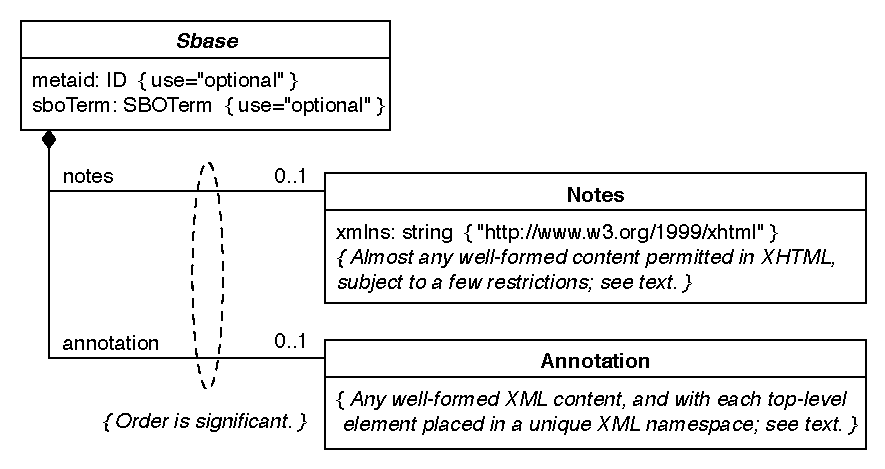
\includegraphics[scale=0.8]{figs/sbase-uml}
  \caption{\changed{The definition of \SBase.  Please refer to
    Section~\protect\ref{sec:notation} for a summary of the UML
    notation used here.  Note that the order of appearance of
    subelements \token{notes} and \token{annotation} is
    significant in instances of objects derived from
    \abstractclass{SBase}: \token{notes} must always come before
    \token{annotation}.  (This requirement arises from
    \xmlschemaone.)}}
  \label{fig:sbase}
\end{figure}

\SBase contains \changed{two attributes and two subelements}, all of which are optional:
\token{metaid}, \token{sboTerm}, \token{notes} and
\token{annotation}.  These are discussed separately in the
following subsections.


\subsubsection{The \token{metaid} \changed{attribute}}
\label{sec:metaid}

The \token{metaid} \changed{attribute} is present for supporting metadata
annotations using RDF~\citep[Resource Description
Format;][]{lassila:1999}.  It has a data type of XML \token{ID}
(the XML identifier type\changed{; see Section~\ref{sec:id}}), which means each \token{metaid} value
must be globally unique within an SBML file.  The \token{metaid}
value serves to identify a model component for purposes such as
referencing that component from metadata placed within
\token{annotation} \changed{elements} (see
Section~\ref{sec:annotation-use}).  Such metadata can use RDF
\token{description} elements, in which an RDF attribute called
\changed{\val{rdf:about} points to} the \token{metaid} identifier of an
object defined in the SBML model.  This topic is discussed in
greater detail in Section~\ref{sec:annotation-standard}.


\subsubsection{\changed{The \token{sboTerm} \changed{attribute}}}
\label{sec:sbase-sboterm}

The \changed{attribute} called \token{sboTerm} is provided on \SBase to support
the use of the Systems Biology Ontology (SBO; see
Section~\ref{sec:sbo}).  \changed{When a value is
given to this attribute, it} must conform to the data type
\primtype{SBOTerm} (Sections~\ref{sec:sboterm-type}).  SBO terms
are a type of optional annotation, and each different class of
SBML object derived from \SBase imposes its own requirements about
the values permitted for \token{sboTerm}.  Specific details on the
permitted values are provided with the definitions of SBML classes
throughout this specification document, and a broader discussion
is provided in Section~\ref{sec:sbo}.


\subsubsection{The \token{notes} \changed{element}}
\label{sec:notes}

The \changed{element} \token{notes} in \SBase is a container for
XHTML~1.0~\citep{pemberton:2002} content.  It is intended to serve
as a place for storing optional information intended to be seen by
humans.  An example use of the \token{notes} \changed{element} would be to
contain formatted user comments about the model \changed{element} in which
the \token{notes} \changed{element} is enclosed.  Every object derived
directly or indirectly from type \SBase can have a separate value
for \token{notes}, allowing users considerable freedom when adding
comments to their models.

XHTML~1.0 is simply a formulation of HTML~4 in XML~1.0.  This
means the full power of HTML formatting is available for use in
\token{notes} content.  The intention behind requiring XHTML
(rather than, for example, plain HTML or plain text) for
\token{notes} content is to balance several conflicting goals: (1)
choosing a format for notes that is compatible with the XML form of
SBML (plain HTML would not be); (2) supporting an international
formatting standard so that users have more control over the
appearance of notes and can predict to some degree how their notes
will be displayed in different tools and environments (which
argues against using plain-text notes); and (3) achieving these
goals using an approach that is hopefully easy enough for software
developers to support using off-the-shelf programming libraries.
It is worth noting in passing that the requirement for XHTML does
not \emph{prevent} users from entering plain-text content with
simple space/tab/newline formatting: it merely requires using the
standard \token{<pre>}...\token{</pre>} element of (X)HTML.

Modern libraries for displaying and editing (X)HTML content are
commonly available in contemporary software programming
environments, and software developers may wish to avail themselves
of these facilities rather than implementing their own XHTML
support systems.


\paragraph{XML namespace requirements for \token{notes}}

The XML content of \token{notes} elements must declare the use of
the XHTML XML namespace.  This can be done in multiple ways.  One
way is to place a namespace declaration for the appropriate
namespace URI (which is \uri{http://www.w3.org/1999/xhtml}) on the
top-level \Sbml object (see Section~\ref{sec:sbml}) and then
reference the namespace in the \token{notes} content using a
prefix.  The following example illustrates this approach:

\begin{example}
<sbml xmlns="http://www.sbml.org/sbml/level2/version\changed{2}" level="2" version="\changed{3}"
      xmlns:xhtml="http://www.w3.org/1999/xhtml">
  ...
  <notes>
    <xhtml:body>
      <xhtml:center><xhtml:h2>A Simple Mitotic Oscillator</xhtml:h2></xhtml:center>
      <xhtml:p>A minimal cascade model for the mitotic oscillator
      involving cyclin and cdc2 kinase</xhtml:p>
    </xhtml:body>
  </notes>
  ...
\end{example}

Another approach is to declare the XHTML namespace within the
\token{notes} content itself, as in the following example:

\begin{example}
...
<notes>
  <body xmlns="http://www.w3.org/1999/xhtml">

    <center><h2>A Simple Mitotic Oscillator</h2></center>

    <p>A minimal cascade model for the mitotic oscillator
    involving cyclin and cdc2 kinase</p>

  </body>
</notes>
...
\end{example}

The \token{xmlns="http://www.w3.org/1999/xhtml"} declaration on
\token{body} as shown above changes the default XML namespace
within it, such that all of its content is by default in the XHTML
namespace.  This is a particularly convenient approach because it
obviates the need to prefix every element with a namespace prefix
(\changed{\ie \token{xhtml:}} in the previous case).  Other
approaches are also possible.


\paragraph{The content of \token{notes}}

SBML does not require the content of \token{notes} to be any
particular XHTML element; the content can be almost any
well-formed XHTML content.  There are only two simple
restrictions.  The first restriction comes from the requirements
of XML: the \token{notes} element must not contain an XML
declaration nor a DOCTYPE declaration.  That is, \token{notes}
must \emph{not} contain

\begin{example}
<?xml version="1.0" encoding="UTF-8"?>  
\end{example}

nor (where the following is only one specific example of a
DOCTYPE declaration)

\begin{example}
<!DOCTYPE html PUBLIC "-//W3C//DTD XHTML 1.0 Strict//EN"
 "http://www.w3.org/TR/xhtml1/DTD/xhtml1-strict.dtd">
\end{example}

The second restriction is intended to balance freedom of content
with the complexity of implementing software that can interpret
the content.  The content of \token{notes} in SBML can consist
only of the following possibilities:
\begin{enumerate}
  
\item A complete XHTML document (minus the XML and DOCTYPE
  declarations, of course), that is, XHTML content beginning with
  the \token{html} tag.  The following is an example skeleton:
  \begin{example}
<notes>
    <html xmlns="http://www.w3.org/1999/xhtml">
      ...
    </html>
</notes>\end{example}

\item The \token{body} element from an XHTML document.  The
  following is an example skeleton:
  \begin{example}
<notes>
    <body xmlns="http://www.w3.org/1999/xhtml">
      ...
    </body>
</notes>\end{example}
  
\item Any XHTML content that would be permitted within a
  \token{body} element.  \changed{If} this consists of multiple
  elements, each one must declare the XML namespace separately.
  The following is an example \changed{fragment}:
  \begin{example}
<notes>
    <p xmlns="http://www.w3.org/1999/xhtml">
      ...
    </p>
    <p xmlns="http://www.w3.org/1999/xhtml">
      ...
    </p>
</notes>\end{example}

\end{enumerate}

Another way to summarize the restrictions above is simply to say
that the content of an SBML \token{notes} element can be only be a
complete \token{html} element, a \token{body} element, or whatever
is permitted inside a \token{body} element.  In practice, this
does not limit in any meaningful way what can be placed inside a
\token{notes} element; for example, if an application or modeler
wants to put a complete XHTML page, including a \token{head}
element, it can be done by putting in everything starting with the
\token{html} container.  However, the restrictions above do make
it somewhat simpler to write software that can read and write the
\token{notes} content.  Appendix~\ref{apdx:processing-notes}
describes one possible approach to doing just that.


\subsubsection{The \token{annotation} \changed{element}}
\label{sec:annotation-use}

Whereas the \token{notes} \changed{element} described above is a container for
content to be shown directly to humans, the \token{annotation}
\changed{element} is a container for optional software-generated content
\emph{not} meant to be shown to humans.  Every object derived
from \SBase can have its own value for \token{annotation}.  The
\changed{element's content} type is XML type \token{any}, allowing essentially
arbitrary \changed{well-formed XML} data content.  SBML places only a few restrictions on
the organization of the content; these are intended to help
software tools read and write the data as well as help reduce
conflicts between annotations added by different tools.


\paragraph{The use of XML namespaces in \token{annotation}}

% FIXME 2006-03-19:
% we should mention that RDF is an additional thing that can show
% up in annotations.  basically what's happening here is that we're
% saying any/all rdf content must be lumped together in one place

At the outset, software developers should keep in mind that
multiple software tools may attempt to read and write annotation
content.  To reduce the potential for collisions between
annotations written by different applications, \sbmltwothree
stipulates that tools must use XML namespaces~\citep{bray:1999} to
specify the intended vocabulary of every annotation.  The
application's developers must choose a URI (\emph{Universal
  Resource Identifier}; \citealt{harold:2001,w3c:2000}) reference
that uniquely identifies the vocabulary the application will use,
and a prefix string for the annotations.  Here is an example.
Suppose an application uses the URI \uri{http://www.mysim.org/ns}
and the prefix \token{mysim} when writing annotations related to
screen layout.  The content of an annotation might look like the
following:

\begin{example}
<annotation>
    <mysim:nodecolors xmlns:mysim="http://www.mysim.org/ns"
         mysim:bgcolor="green" mysim:fgcolor="white"/>
</annotation>
\end{example}

In this particularly simple \changed{example}, the content consists of a single
XML element (\token{nodecolors}) with two attributes
(\token{bgcolor}, \token{fgcolor}), all of which are prefixed by
the string \token{mysim}.  (Presumably this particular content
would have meaning to the hypothetical application in question.)
The content in this particular example is small, but it should be
clear that there could easily have been an arbitrarily large
amount of data placed inside the \token{mysim:nodecolors} element.

The key point of the example above is that application-specific
annotation data is entirely contained inside a single
\emph{top-level element} within the SBML \token{annotation}
container.  SBML Level~2 Version~\changed{3} places the following
restrictions on annotations:
\begin{itemize}

\item Within a given SBML \token{annotation} element, there can
  only be one top-level element using a given namespace.  An
  annotation element can contain multiple top-level elements but
  each must be in a different namespace.

\item No top-level element in an \token{annotation} may use an
  SBML XML namespace, either explicitly by referencing one of the
  SBML XML namespace URIs or implicitly by failing to specify any
  namespace on the annotation.  \changed{As of \sbmltwothree, the
    defined SBML namespaces are the following URIs:}
  \begin{itemize}\setlength{\parskip}{-0.2ex}
  \item \uri{http://www.sbml.org/sbml/level1}
  \item \uri{http://www.sbml.org/sbml/level2}
  \item \uri{http://www.sbml.org/sbml/level2/version2}
  \item \changed{\uri{http://www.sbml.org/sbml/level2/version3}}
  \end{itemize}
  
\item The ordering of top-level elements within a given
  \token{annotation} element is \emph{not} significant.  An
  application should not expect that its annotation content
  appears first in the \token{annotation} element, nor in any
  other particular location.  \changed{Moreover, the ordering of
    top-level annotation elements may be changed by}
  \changed{different applications as they read and write the same
    SBML file.}

\end{itemize}

The use of XML namespaces in this manner is intended to improve
the ability of multiple applications to place annotations on SBML
model \changed{elements} with reduced risks of interference or name
collisions.  Annotations stored by different simulation packages
can therefore coexist in the same model definition.  The rules
governing the content of \token{annotation} elements are designed
to enable applications to easily add, change, and remove their
annotations from SBML elements while simultaneously preserving
annotations inserted by other applications when mapping SBML from
input to output.

\begin{blockChanged}

As a further simplification for developers of software and to
improve software interoperability, applications are only required
to preserve other annotations (i.e., annotations they do not
recognize) when those annotations are self-contained entirely
within \token{annotation}, complete with namespace declarations.
The following is an example:

\begin{example}
<annotation>
    <topLevelElement xmlns:"URI">
       \textrm{\emph{... content in the namespace identified by \textquotedblleft{}URI\textquotedblright}...}
    </topLevelElement>
</annotation>
\end{example}

\end{blockChanged}

Some more examples hopefully will make \changed{these points} more clear.  The next
example is invalid because it contains a top-level element in the
SBML XML namespace---this happens because no namespace is declared
for the \token{<cytoplasm>} element, which means by default it
falls into the \changed{enclosing} SBML namespace:

\begin{example}
<annotation>
    <cytoplasm/>
</annotation>
\end{example}

The following example is \changed{also} invalid, \changed{this
  time} because it contains two top-level elements using the same
XML namespace.  Note that it does not matter that these are two
different top-level elements (\token{<nodecolors>} and
\token{<textcolors>}); what matters is that these separate
elements are both in the same namespace rather than having been
collected and placed inside one overall container element for that
namespace.

\begin{example}
<annotation>
    <mysim:nodecolors xmlns:mysim="http://www.mysim.org/ns"
        mysim:bgcolor="green" mysim:fgcolor="white"/>
    <mysim:textcolors xmlns:mysim="http://www.mysim.org/ns"
        mysim:bgcolor="green" mysim:fgcolor="white"/>
</annotation>
\end{example}

On the other hand, the following example is valid:

\begin{example}
<annotation>
    <mysim:geometry xmlns:mysim="http://www.mysim.org/ns"
             mysim:bgcolor="green" mysim:fgcolor="white">
        <graph:node xmlns:graph="http://www.graph.org/ns" 
             graph:x="4" graph:y="5" />
    </mysim:geometry>
    <othersim:icon xmlns:othersim="http://www.othersim.com/">
        WS2002
    </othersim:icon>
</annotation>
\end{example}

\begin{blockChanged}

For completeness, we note that annotations can legally be empty:

\begin{example}
<annotation />
\end{example}

\end{blockChanged}

It is worth keeping in mind that although XML namespace names must
be URIs, they are (like all XML namespace names) \emph{not
  required} to be directly usable in the sense of identifying an
actual, retrieval document or resource on the
Internet~\citep{bray:1999}.  URIs such as
\uri{http://www.mysim.org/} may appear as though they are (\eg)
Internet addresses, but there are not the same thing.  This style
of URI strings, using a domain name and other parts, is only a
simple and commonly-used way of creating a unique name string.

Finally, note that the namespaces being referred to here are XML
namespaces specifically in the context of the \token{annotation}
\changed{element} on \SBase.  The namespace issue here is unrelated to the
namespaces discussed in Section~\ref{sec:identifiers} in the
context of component identifiers in SBML.


\paragraph{Content of annotations and implications for software tools}

The \token{annotation} \changed{element} in the definition of \SBase exists in
order that software developers may attach optional
application-specific data to the \changed{elements} in an SBML model.
However, it is important that this facility not be misused.  In
particular, it is \emph{critical} that data essential to a model
definition or that can be encoded in existing SBML \changed{elements} is
\emph{not} stored in \token{annotation}. Parameter values,
functional dependencies between model \changed{elements}, etc., should not
be recorded as annotations.  It is crucial to keep in mind the
fact that data placed in annotations can be freely ignored by
software applications.  If such data affects the interpretation of
a model, then software interoperability is greatly impeded.

Here are examples of the kinds of data that may be appropriately
stored in \token{annotation}: (a) information about the graphical
layout of model components; (b) application-specific processing
instructions that do not change the essential meaning of a model;
(c) identification information for cross-referencing components in
a model with items in a data resource such as a database\changed{;
  and (d) information about the model that cannot} \changed{be
  readily encoded in existing SBML elements.}


\paragraph{Standardized format for certain classes of annotations}

\begin{blockChanged}

For case (c) above (i.e., cross-references between model
components and data resources, \sbmltwothree recommends a
standard format for use within \token{annotation}
\changed{elements}.  It should be used in preference to
proprietary syntaxes to maximize the likelihood that multiple
software tools will converge on the same syntax for this kind of
information.  The recommended scheme is described in
Section~\ref{sec:finney-novere}.

\end{blockChanged}


%-----------------------------------------------------------------------------
\subsection{The \token{id} and \token{name} \changed{attributes} on SBML components}
\label{sec:idnameattribs}
%-----------------------------------------------------------------------------

As will become apparent below, most \changed{objects} in SBML include two
common \changed{attributes}: \token{id} and \token{name}.  These \changed{attributes} are not
defined on \SBase (as explained in
Section~\ref{sec:why-not-on-sbase} below), but where they do
appear, the common rules of usage described below apply.


\subsubsection{The \token{id} \changed{attribute} and identifier scoping}
\label{sec:identifiers}

The \token{id} \changed{attribute is mandatory on most objects} in
SBML.  It is used to identify a component within the model
definition.  Other SBML \changed{objects} can refer to the component
using this identifier.  The data type of \token{id} is always
either \primtype{Sid} (Section~\ref{sec:sid}) or
\primtype{UnitSId} (Section~\ref{sec:unitsid}), depending on the
object in question.

A model can contain a large number of components representing
different parts.  This leads to a problem in deciding the scope of
an identifier: in what contexts does a given identifier \emph{X}
represent the same thing?  The approaches used in existing
simulation packages tend to fall into two categories which we may
call global and local.  The \emph{global} approach places all
identifiers into a single global space of identifiers, so that an
identifier \emph{X} represents the same thing wherever it appears
in a given model definition.  The \emph{local} approach places
symbols in separate identifier namespaces, depending on the
context, where the context may be, for example, individual
reaction rate expressions.  The latter approach means that a user
may use the same identifier \emph{X} in different rate expressions
and have each instance represent a different quantity.

The fact that different simulation programs may use different
rules for identifier resolution poses a problem for the exchange
of models between simulation tools.  Without careful
consideration, a model written out in SBML format by one program
may be misinterpreted by another program.  \sbmltwo must therefore
include a specific set of rules for treating identifiers and their
scopes.

The scoping rules in \sbmltwo are relatively
straightforward and are intended to avoid this problem with a
minimum of requirements on the implementation of software tools:
\begin{itemize}
  
\item The identifier (\ie the value of the \changed{attribute} \token{id}) of
  every \FunctionDefinition, \CompartmentType, \SpeciesType,
  \Compartment, \Species, \Parameter, \Reaction,
  \SpeciesReference, \ModifierSpeciesReference, \Event, and
  \Model, must be unique across the set of all such identifiers in
  the model.  This means, for example, that a reaction and a
  species definition cannot both have the same identifier.

\item The identifier of every \UnitDefinition must be unique
  across the set of all such identifiers in the model.  However,
  unit identifiers live in a separate space of identifiers from
  other identifiers in the model\changed{, by} \changed{virtue of
    the fact that the data type of unit identifiers is
    \primtype{UnitSId} (Section~\ref{sec:unitsid}) and not
    \primtype{SId}}.
  
\item Each \Reaction instance (see Section~\ref{sec:reactions})
  establishes a separate private local space for local \Parameter
  identifiers.  Within the definition of that reaction, local
  parameter identifiers override (shadow) identical identifiers
  outside of that reaction.  Of course, the corollary of this is
  that local parameters inside a \Reaction object instance are not
  visible to other objects outside of that reaction.

\end{itemize}
The set of rules above can enable software packages using either
local or global identifier spaces for parameters to exchange SBML
model definitions.  Software systems using local identifiers for
parameters internally should, in principle, be able to accept SBML
model definitions without needing to change component identifiers.
Environments using a common global space of identifiers for
parameters internally can perform manipulations of the identifiers
of local parameters within reaction definitions to avoid
identifier collisions.

The guidelines described here will hopefully provide a clean
transition path to future levels of SBML, when submodels are
introduced (Section~\ref{sec:level-3}).  Submodels will provide
the ability to compose one model from a collection of other
models.  This capability will have to be built on top of
\sbmltwo's namespace organization.  A straightforward approach to
handling namespaces is to make each submodel's space be private.
The rules governing identifier scoping within a submodel can
simply be the Level~2 namespace rule described here, with each
submodel having its own (to itself, global) namespace.


\subsubsection{The \token{name} \changed{attribute}}
\label{sec:name}

In contrast to the \token{id} \changed{attribute}, the \token{name} \changed{attribute} is
optional and is not intended to be used for cross-referencing
purposes within a model.  Its purpose instead is to provide a
human-readable label for the component.  The data type of 
\token{name} is the type \primtype{string} defined in XML
Schema~\citep{biron:2000,thompson:2000} and discussed further in
Section~\ref{sec:primitive-types}.  SBML imposes no restrictions
as to the content of \token{name} \changed{attributes} beyond those restrictions
defined by the \primtype{string} type in XML Schema.

The recommended practice for handling \token{name} is as follows.
If a software tool has the capability for displaying the content
of \token{name} \changed{attributes}, it should display this content to the user
as a component's label instead of the component's \token{id}.
If the user interface does not have this capability (e.g.,
because it cannot display or use special characters in symbol
names), or if the \token{name} \changed{attribute} is missing on a given
component, then the user interface should display the value of the
\token{id} \changed{attribute} instead.  (Script language interpreters are
especially likely to display \token{id} \changed{instead of}
\token{name}.)

As a consequence of the above, authors of systems that
automatically generate the values of \token{id} \changed{attributes} should be
aware some systems may display the \token{id}'s to the user.
Authors therefore may wish to take some care to have their
software create \token{id} values that are: (a) reasonably easy
for humans to type and read; and (b) likely to be meaningful, \eg
the \token{id} \changed{attribute} is an abbreviated form of the name \changed{attribute} value.

An additional point worth mentioning is although there are
restrictions on the uniqueness of \token{id} values (see
Section~\ref{sec:identifiers} above), there are no restrictions on
the uniqueness of \token{name} values in a model.  This allows
software packages leeway in assigning component identifiers.


\subsubsection{Why \token{id} and \token{name} are not defined on \class{SBase}}
\label{sec:why-not-on-sbase}

% [MH 2006-03-06] Most of the following issues could be addressed
% by having a separate "SBaseWithId" class.  I think only the first
% two reasons couldn't be addressed.  Thus, the original paragraph
% (which only talked about scoping) was almost in some sense the
% fundamental reason.  I added this other stuff to address some
% questions made in the past, but these other arguments are all
% trumped by saying ``just define an SBaseWithID''.  Therefore,
% it may be worth thinking about going back to the single reason.

Although many SBML components \changed{feature}
\token{id} and \token{name}, these \changed{attributes} are purposefully not defined on
\SBase.  There are several reasons for this.
\begin{itemize}
  
\item The presence of an SBML identifier \changed{attribute} (\token{id})
  necessarily requires specifying scoping rules for the
  corresponding identifiers.  However, the \SBase abstract type is
  used as the basis for defining components whose scoping rules
  are in some cases different from each other.  (See
  Section~\ref{sec:identifiers} for more details).  If \SBase were
  to have an \token{id} \changed{attribute}, then the specification of \SBase
  would need a default scoping rule and this would then have to be
  overloaded on derived classes that needed different scoping.
  This would make the SBML specification \changed{even more} complex.
  
\item Identifier are optional on some SBML components and required
  on most others.  If \token{id} were defined as optional on
  \SBase, most component classes would separately have to redefine
  \token{id} as being mandatory---hardly an improvement over the
  current arrangement.  Conversely, if \token{id} were defined as
  mandatory on \SBase, it would prevent it from being optional on
  components where it \emph{is} currently optional.
  
\item The \SBase abstract type is used as the base type for
  certain \changed{objects} such as \changed{\Sbml, \AssignmentRule},
  etc., which do not have identifiers because these components do
  not need to be referenced by other components.  If \SBase had a
  mandatory \token{id} \changed{attribute}, \emph{all} objects of
  these other types in a model would then need to be assigned
  unique identifiers.  Similarly, \changed{because \SBase is the
    base type of the \token{listOf\rule{0.5in}{0.5pt}} lists},
  putting \token{id} on \SBase would require all of these lists in
  a model to be given identifiers.  This would be a needless
  burden on software developers, tools, and SBML users, requiring
  them to generate and store additional identifiers for objects
  that never need them.
  
\item \SBase does not have a \token{name} simply because such an
  \changed{attribute} is always paired with an \token{id}.  Without
  \token{id} on \SBase, it does not make sense to have
  \token{name}.

\end{itemize}


%-----------------------------------------------------------------------------
\subsection{Mathematical formulas in SBML Level 2}
\label{sec:formulas}
%-----------------------------------------------------------------------------

Mathematical expressions in SBML Level~2 are represented using
\mathmltwo~\citep{w3c:2000b}.  MathML is an international standard
for encoding mathematical expressions using XML.  There are two
principal facets of MathML, one for encoding content (\ie the
semantic interpretation of a mathematical expression), and another
for encoding presentation or display characteristics.  SBML only
makes direct use of a subset of the content portion of MathML.  By
borrowing a separately-developed XML standard, we can avoid having
to define a specialized syntax for mathematical expressions in
SBML and simultaneously leverage existing intellectual and
technological work already done in the MathML community.  However,
it is not possible to produce a completely smooth and
conflict-free interface between MathML and other standards used by
SBML (in particular, \xmlschema).  Two specific issues and their
resolutions are discussed in Sections~\ref{sec:cn-token}.

The XML namespace URI for all MathML elements is
\uri{http://www.w3.org/1998/Math/MathML}.  Everywhere MathML
content is allowed in SBML, the MathML elements must be properly
placed within the \mathmltwo namespace.  In XML, this can be
accomplished in a number of ways, and the examples throughout this
specification illustrate the use of this namespace and MathML in
SBML.  Please refer to the W3C document by \citet{bray:1999} for
more technical information about using XML namespaces.


\subsubsection{Subset of MathML used in SBML Level 2}
\label{sec:mathmlsubset}

The subset of \mathmltwo elements used in SBML Level~2 is similar
to that used by CellML~\citep{hedley:2001b}, another model
definition language with similar goals as SBML.  The subset of
MathML elements used in SBML is listed below:
\begin{itemize}\setlength{\parskip}{-0.2ex}

\item \emph{token}: \token{cn}, \token{ci}, \token{csymbol},
  \token{sep}
  
\item \emph{general}: \token{apply}, \token{piecewise},
  \token{piece}, \token{otherwise}, \token{lambda} (the last is
  restricted to use in \FunctionDefinition)

\item \emph{relational operators}: \token{eq}, \token{neq},
  \token{gt}, \token{lt}, \token{geq}, \token{leq}

\item \emph{arithmetic operators}: \token{plus}, \token{minus},
  \token{times}, \token{divide}, \token{power}, \token{root},
  \token{abs}, \token{exp}, \token{ln}, \token{log},
  \token{floor}, \token{ceiling}, \token{factorial}

\item \emph{logical operators}: \token{and}, \token{or},
  \token{xor}, \token{not}

\item \emph{qualifiers}: \token{degree}, \token{bvar},
  \token{logbase}

\item \emph{trigonometric operators}: \token{sin}, \token{cos},
  \token{tan}, \token{sec}, \token{csc}, \token{cot},
  \token{sinh}, \token{cosh}, \token{tanh}, \token{sech},
  \token{csch}, \token{coth}, \token{arcsin}, \token{arccos},
  \token{arctan}, \token{arcsec}, \token{arccsc}, \token{arccot},
  \token{arcsinh}, \token{arccosh}, \token{arctanh},
  \token{arcsech}, \token{arccsch}, \token{arccoth}

\item \emph{constants}: \token{true}, \token{false},
  \token{notanumber}, \token{pi}, \token{infinity},
  \token{exponentiale}

\item \emph{annotation}: \token{semantics}, \token{annotation},
  \token{annotation-xml}

\end{itemize}
\vspace*{-0.75ex}
The inclusion of logical operators, relational operators,
\token{piecewise}, \token{piece}, and \token{otherwise} elements
facilitates the encoding of discontinuous expressions.  Note that
MathML elements for representing partial differential calculus are
not included.  We anticipate that the requirements for partial
differential calculus will be addressed in proposals for future
SBML geometry representations (see Section~\ref{sec:level-3}).

As defined by \mathmltwo, the semantic interpretation of the
mathematical functions listed above follows the definitions of the
functions laid out by \cite{abramowitz:1997} and
\cite{zwillinger:1988}.  Readers are directed to these sources and
the MathML specification for information about such things as
which principal values of the inverse trigonometric functions to
use.

Software authors should take particular note of the MathML
semantics of the N-ary operators \token{plus}, \token{times},
\token{and}, \token{or} and \token{xor}, when they are used with
different numbers of arguments.  The MathML
specification~\citep{w3c:2000b} appendix C.2.3 describes the
semantics for these operators with zero, one, and more arguments.

The following are the only attributes permitted on MathML elements
in SBML (in addition to the \token{xmlns} attribute on
\token{math} elements):
\begin{itemize}\setlength{\parskip}{-0.2ex}

\item \token{style}, \token{class} and \token{id} on any element;

\item \token{encoding} and \token{definitionURL} on
  \token{csymbol} elements; and

\item \token{type} on \token{cn} elements.

\end{itemize}\vspace*{-0.75ex}
Missing values for these attributes are to be treated in the same
way as defined by MathML.  These restrictions on attributes are
designed to confine the MathML elements to their default semantics
and to avoid conflicts in the interpretation of the type of token
elements.


\subsubsection{Numbers and \token{cn} elements}
\label{sec:cn-token}
\label{sec:mathml-value-space}

In MathML, literal numbers are written as the content portion of a
particular element called \token{cn}.  This element takes an
optional attribute, \token{type}, used to indicate the \emph{type}
of the number (such as whether it is meant to be an integer or a
floating-point quantity).  Here is an example of its use:
\begin{example}
<math xmlns="http://www.w3.org/1998/Math/MathML">
    <apply>
        <times/> <cn type="integer"> 42 </cn> <cn type="real"> 3.3 </cn>
    </apply>
</math>
\end{example}

The content of a \token{cn} element must be a number.  The number
can be preceded and succeeded by whitespace (see
Section~\ref{sec:mathml-whitespace}).  The following are the only
permissible values for the \token{type} attribute on MathML
\token{cn} elements: \val{e-notation}, \val{real}, \val{integer},
and \val{rational}.  The value of the \token{type} attribute
defaults to \val{real} if it is not specified on a given
\token{cn} element.


\paragraph{Value space restrictions on \token{cn} content}

SBML imposes certain restrictions on the value space of numbers
allowed in MathML expressions.  According to the \mathmltwo
specification, the values of the content of \token{cn} elements do
not necessarily have to conform to any specific floating point or
integer representations designed for CPU implementation.  For
example, in strict MathML, the value of a \token{cn} element could
exceed the maximum value that can be stored in a IEEE 64 bit
floating point number (IEEE 754).  This is different from the XML
Schema type \primtype{double} that is used in the definition of
floating point \changed{attributes} of \changed{objects} in SBML; the XML Schema
\primtype{double} \emph{is} restricted to IEEE double-precision
64-bit floating point type IEEE 754-1985.  To avoid an
inconsistency that would result between numbers elsewhere in SBML
and numbers in MathML expressions, \sbmltwothree imposes the
following restriction on MathML content appearing in SBML:
\begin{itemize}
  
\item Integer values (\ie the \changed{values} of \token{cn} elements
  having \token{type}=\val{integer} \changed{and both values in \token{cn} elements}
  \changed{having \token{type}=\val{rational}}) must conform to the
  \primtype{int} type used elsewhere in SBML
  (Section~\ref{sec:integer})
  
\item Floating-point values (\ie the content of \token{cn}
  elements having \token{type}=\val{real} or
  \token{type}=\val{e-notation}) must conform to the
  \primtype{double} type used elsewhere in SBML
  (Section~\ref{sec:double})
\end{itemize}


\paragraph{Syntactic differences in the representation of numbers
  in scientific notation}

It is important to note that MathML uses a style of scientific
notation that differs from what is defined in XML Schema, and
consequently what is used in SBML attribute values.  The
\mathmltwo type \val{e-notation}
\changed{(as} \changed{well as the type \val{rational})}
requires the mantissa and
exponent to be separated by one \texttt{<sep/>} element.  The
mantissa must be a real number and the exponent part must be a
signed integer.  This leads to expressions such as

\begin{example}
<cn type="e-notation"> 2 <sep/> -5 </cn>
\end{example}

for the number $2 \times 10^{-5}$.  It is especially
important to note that the expression

\begin{example}
<cn type="e-notation"> 2e-5 </cn>
\end{example}

is \emph{not valid} in \mathmltwo and therefore cannot be used in
MathML content in SBML.  However, elsewhere in SBML, when an
attribute value is declared to have the data type
\primtype{double} (a type taken from XML Schema), the compact
notation \val{2e-5} is in fact allowed.  In other words, within
MathML expressions contained in SBML (and \emph{only} within such
MathML expressions), numbers in scientific notation must take the
form \token{<cn type="e-notation"> 2 <sep/> -5 </cn>}, and
everywhere else they must take the form \val{2e-5}.

This is a regrettable difference between two standards that SBML
replies upon, but it is not feasible to redefine these types
within SBML because the result would be incompatible with parser
libraries written to conform with the MathML and XML Schema
standards.  It is also not possible to use XML Schema to define a
data type for SBML attribute values permitting the use of the
\token{<sep/>} notation, because XML attribute values cannot
contain XML elements---that is, \token{<sep/>} cannot appear in an
XML attribute value.


\begin{blockChanged}

\paragraph{Units of numbers in MathML \token{cn} expressions}
\label{sec:units-of-mathml}

What units should be attributed to values appearing inside MathML
\token{cn} elements?  One answer is to assume that the units
should be ``whatever units appropriate in the context where the
number appears''.  This implies that units can always be assigned
unambiguously to any number by inspecting the expression in which
it appears, and this
turns out to be false.  Another answer is that numbers should be
considered ``dimensionless''.  This may be correct in pure
mathematics and other contexts, but it turns out that when numbers
appear in expressions in SBML's domain of application, they are
rarely \emph{intended} to have the units \val{dimensionless} even
if the units are not declared: they are \emph{supposed} to have
specific units, but the units are \changed{usually undeclared.  (Being}
\changed{``dimensionless'' is} not the same as having
\emph{undeclared} units!)  If SBML defined
numbers as being \emph{by default} dimensionless, it would likely
result in many models being technically incorrect without the
modeler being aware of it unless their software tools performed
dimensional analysis.  Most software tools today still do not, and
so the discovery of incorrect units would not occur until other
researchers and database curators attempted to use the model in
software packages that did check units.

The current approach in SBML is to leave the default units of
numbers undefined.  Software packages and modelers are encouraged
to explicitly add unit declarations to numbers; such declarations
can permit software tools to perform dimensional analysis and
potentially report model errors.  There are (at least) two simple
methods for associating units with numerical quantities in SBML:

\begin{itemize}

\item Do not use literal numbers at all; instead, define
  \Parameter objects (Section~\ref{sec:parameters}) for every
  quantity, and declare units for each such parameter in its
  definitions.  (This is the best modeling practice anyway.)

\item Define separate parameters for the needed units, such that
  the parameters have numerical values of \val{1} and the
  appropriate units assigned via their \token{units} attribute.
  Parameters are described in detail in
  Section~\ref{sec:parameters}, but to foreshadow them, here is an
  example:
  \begin{example}
    <listOfParameters>
        <parameter id="SubstanceUnits" value="1" units="substance"/>
    </listOfParameters>\end{example}

  Numbers that need to be in the model's substance units can then
  be assigned those units by multiplying the number with the
  parameter defined above using standard MathML.  The numerical
  value will be left unchanged because the value of the parameter
  is the multiplicative identity \val{1}.  For example:
  \begin{example}
    <apply>
        <times/>
        <cn> 2 </cn>
        <ci> SubstanceUnits </ci>
    </apply>\end{example}\vspace*{-1ex}

\end{itemize}

\end{blockChanged}


\subsubsection{Use of \token{ci} elements in MathML expressions in SBML}
\label{sec:ci-token}

The content of a \token{ci} element must be an SBML identifier
that is declared elsewhere in the model.  The identifier can be
preceded and succeeded by whitespace. The set of possible
identifiers that can appear in a \token{ci} element depends on the
containing \changed{element} in which the \token{ci} is used:
\begin{itemize}
  
\item If a \token{ci} element appears in the body of a
  \FunctionDefinition object
  (Section~\ref{sec:functiondefinition}), the referenced
  identifier must be either (i) one of the declared arguments to
  that function, or (ii) the identifier of a previously defined
  \changed{\FunctionDefinition object} in the model.
  
\item Otherwise, the referenced identifier must be that of a
  \Species, \Compartment, \Parameter, \FunctionDefinition, or
  \Reaction object defined in the model.  The following are the
  only possible interpretations of using such an identifier in
  SBML:
  \begin{itemize}
    
  \item \emph{Species identifier}: When a \Species identifier
    occurs in a \token{ci} element, it represents the quantity of
    that species in terms of either \quantity{amount of substance}
    units or in terms of \quantity{concentration} units, depending
    on the definition of that species; see
    Section~\ref{sec:species-units}.
    
  \item \emph{Compartment identifier}: When a \Compartment
    identifier occurs in a \token{ci} element, it represents the
    size of the compartment.  The units associated with the size
    of the compartment are those given on the \Compartment
    \changed{element} that declares the identifier; see
    Section~\ref{sec:compartment-units}.
    
  \item \emph{Parameter identifier}: When a \Parameter identifier
    occurs in a \token{ci} element, it represents the numerical
    value assigned to that parameter.  The units associated with
    the parameter's value are the units assigned in the instance
    of the \Parameter \changed{element}; see
    Section~\ref{sec:parameter-units}.
    
  \item \emph{Function identifier}: When a \FunctionDefinition
    identifier occurs in a \token{ci} element, it represents a
    call to that function.  Function references in MathML occur in
    the context of using MathML's \token{apply} and often involve
    supplying arguments to the function; see
    Section~\ref{sec:functiondefinition}.  \changed{The units
      associated} \changed{with the value returned by the function
      call are the overall units of the mathematical expression}
      \changed{contained in the function definition.}
    
  \item \emph{Reaction identifier}: When a \Reaction identifier
    occurs in a \token{ci} element, it represents the rate of that
    reaction as determined by the mathematical formula in the
    \KineticLaw object within the \Reaction.  The units associated
    with the reaction are \quantity{substance}/\quantity{time},
    with the \quantity{substance} and \quantity{time} units
    established by the values of the SBML built-in units
    \val{substance} and \val{time}, respectively.  These units may
    be redefined in model; see Section~\ref{sec:built-in-units}.
    If the reaction definition has no \KineticLaw, the use of the
    reaction identifier is an error (perhaps indicating that the
    model is incomplete).

  \end{itemize}

\end{itemize}

The content of \token{ci} elements in MathML formulas outside of a
\KineticLaw or \FunctionDefinition must always refer to objects
declared in the top level global namespace; \ie SBML uses ``early
binding'' semantics.  Inside of \KineticLaw, a \token{ci} element
can additionally refer to local parameters defined within that
\KineticLaw instance; see Section~\ref{subsec:kinetic-law} for
more information.


\begin{blockChanged}

\subsubsection{Interpretation of boolean values}
\label{sec:handling-booleans}

As noted already in Section~\ref{sec:boolean}, there is another
unfortunate difference between the \xmlschemaone and \mathmltwo
standards that impacts mathematical expressions in SBML: in
\xmlschema, the value space of type \primtype{boolean} includes
\val{true}, \val{false}, \val{1}, and \val{0}, whereas in
\mathml, only \val{true} and \val{false} count as boolean
values.

The impact of this difference thankfully is minimal because the
\xmlschema definition is only used for attribute values on SBML
objects, and those values turn out never to be accessible from
\mathml content in SBML---values of boolean \changed{attributes} on SBML objects
can never enter into \mathml expressions.  Nevertheless, software
authors and users should be aware of the difference and in
particular that \val{0} and \val{1} are interpreted as numerical
quantities in mathematical expressions.  There is no automatic
conversion of \val{0} or \val{1} to boolean values in contexts
where booleans are expected.  This allows stricter type checking
and unit verification during the validation of models.

\end{blockChanged}


\subsubsection{Handling of whitespace}
\label{sec:mathml-whitespace}

\mathmltwo defines ``whitespace'' in the same way as XML does, \ie
the space character (Unicode hexadecimal code 0020), horizontal
tab (code 0009), newline or line feed (code 000A), and carriage
return (code 000D).  In MathML, the content of elements such as
\token{cn} and \token{ci} can be surrounded by whitespace
characters.  Prior to using the content, this whitespace is
``trimmed'' from both ends: all whitespace at the beginning and
end of the content is removed~\citep{ausbrooks:2003}.  For
example, in \texttt{<cn> 42 </cn>}, the amount of white space on
either side of the ``\texttt{42}'' inside the \texttt{<cn>}
\ldots\ \texttt{</cn>} container does not matter.  Prior to
interpreting the content, the whitespace is removed altogether.


\subsubsection{Use of \token{csymbol} elements in MathML expressions in SBML}
\label{sec:csymbol-token}

SBML Level 2 uses the MathML \token{csymbol} element to denote
certain built-in mathematical entities without introducing
reserved names into the component identifier namespace.  The
\token{encoding} \changed{attribute} of \token{csymbol} \changed{must} be set to
\val{text}.  The \token{definitionURL} should be set to one of the
following predefined SBML symbol URIs:
\begin{itemize}

\item \uri{http://www.sbml.org/sbml/symbols/time}.  This
  represents the current simulation time.  See
  Section~\ref{sec:meaning-of-time} for more information.  The
  units of the current time entity are determined from the
  built-in \token{time} of Table~\vref{tab:builtin}.

\item \uri{http://www.sbml.org/sbml/symbols/delay}.  This
  represents a delay function.  The delay function has the form
  $delay(x, d)$, taking two MathML expressions as arguments.  Its
  value is the value of argument $x$ at $d$ time units before the
  current time.  There are no restrictions on the form of $x$.
  The units of the $d$ parameter are determined from the built-in
  \token{time}.  The value of the $d$ parameter, when evaluated,
  must be numerical (\ie a number in MathML real, integer, or
  ``e-notation'' format) and be greater than or equal to 0.  The
  \emph{delay} function is useful for representing biological
  processes having a delayed response, but where the detail of the
  processes and delay mechanism is not relevant to the operation
  of a given model.  See Section~\ref{sec:meaning-of-time} below
  for additional considerations surrounding the use of this
  \token{csymbol}.

\end{itemize}

The following examples demonstrate these concepts.  The XML fragment below
encodes the formula $x + t$, where $t$ stands for time.

\begin{example}
<math xmlns="http://www.w3.org/1998/Math/MathML">
    <apply>
        <plus/>
        <ci> x </ci>
        <csymbol encoding="text" definitionURL="http://www.sbml.org/sbml/symbols/time">
            t
        </csymbol>
    </apply>
</math>
\end{example}

In the fragment above, the use of the token \token{t} is mostly a
convenience for human readers---the string inside the
\token{csymbol} could have been almost anything, because it is
essentially ignored by MathML parsers and SBML.  Some MathML and
SBML processors will take note of the token and use it when
presenting the mathematical formula to users, but the token used
has no impact on the interpretation of the model and it does
\emph{not} enter into the SBML component identifier namespace.  In
other words, the SBML model cannot refer to \token{t} in the
example above.  The content of the \token{csymbol} element is for
rendering purposes only and can be ignored by the parser.

As a further example, the following XML fragment encodes the equation
$k + delay(x, 0.1)$ or alternatively $k_t + x_{t - 0.1}$:

\begin{example}
<math xmlns="http://www.w3.org/1998/Math/MathML">
    <apply>
        <plus/>
        <ci> k </ci>
        <apply>
            <csymbol encoding="text" definitionURL="http://www.sbml.org/sbml/symbols/delay">
                delay
            </csymbol>
            <ci> x </ci>
            <cn> 0.1 </cn>
        </apply>
    </apply>
</math>
\end{example}

Note that the URI in the value of \token{definitionURL}, as all
URIs, is intended to serve as a unique identifier and is not
intended to be dereferenced as an Internet address.  There is
nothing actually located at the address
\uri{http://www.sbml.org/sbml/symbols/delay}.


\subsubsection{Simulation time}
\label{sec:meaning-of-time}

The principal use of SBML is to represent quantitative dynamical
models whose behaviors manifest themselves over time.  In defining
an SBML model using constructs such as reactions, time is most
often implicit and does not need to be referred to in the
mathematical expressions themselves.  However, sometimes an
explicit time dependency needs to be stated, and for this purpose,
the \emph{time} \token{csymbol} (described above in
Section~\ref{sec:csymbol-token}) may be used.  This \emph{time}
symbol refers to ``instantaneous current time'' in a simulation,
frequently given the literal name $t$ in one's equations.

An assumption in SBML is that ``start time'' or ``initial time''
in a simulation is zero, that is, if $t_0$ is the initial time in
the system, $t_0 = 0$.  This corresponds to the most common
scenario.  Initial conditions in SBML take effect at time $t = 0$.
There is no mechanism in SBML for setting the initial time to a
value other than 0.  To refer to a different time in a model, one
approach is to define a \Parameter for a new time variable and use
an \AssignmentRule in which the assignment expression subtracts a
value from the \token{csymbol} \emph{time}.  For example, if the
desired offset is 2 time units, the MathML expression would be

\begin{example}
<math xmlns="http://www.w3.org/1998/Math/MathML">
    <apply>
        <minus/>
        <csymbol encoding="text" definitionURL="http://www.sbml.org/sbml/symbols/time"> t
        </csymbol>
        <cn> 2 </cn>
    </apply>
</math>
\end{example}

SBML's assignment rules (Section~\ref{sec:assignmentrule}) can be
used to express mathematical statements that hold true at all
moments, so using an assignment rule with the expression above
will result in the value being equal to $t - 2$ at every point in
time.  A parameter assigned this value could then be used
elsewhere in the model, its value could be plotted by a simulator,
etc.


\subsubsection{Initial conditions and special considerations}
\label{sec:before-t0}

The identifiers of \Species, \Compartment, \Parameter, and
\Reaction object instances in a given SBML model refer to the main
variables in a model.  Depending on certain attributes of these
objects (\eg the \changed{attribute} \token{constant} on species, compartments
and parameters---this and other conditions are explained in the
relevant sections elsewhere in this document), some of the
variables may have constant values throughout a simulation, and
others' values may change.  These changes in values over time are
determined by the system of equations constructed from the model's
reactions, initial assignments, rules, and events.

As described in Section~\ref{sec:meaning-of-time}, an SBML model's
simulation is assumed to begin at $t = 0$.  The availability of
the \emph{delay} \token{csymbol} (Section~\ref{sec:csymbol-token})
introduces the possibility that at $t \geq 0$, mathematical
expressions in a model may draw on values of model components from
time \emph{prior} to $t = 0$.  A simulator may therefore need to
compute the values of variables at time points $t_i \leq 0$ to
allow the calculation of values required for the evaluation of
delay expressions in the model for $t \geq 0$.  If there are no
delays in the model, then $t_i = 0$.

The following is how the definitions of the model should be
applied:
\begin{enumerate}

\item At time $t_i$:
  \begin{itemize}
    
  \item Every \Species, \Compartment, and \Parameter whose
    definition includes an initial value is assigned that value.
    If an \changed{element has} \token{constant}=\val{false}, its
    value may be changed by other constructs or reactions in a
    model according to the steps below; if
    \token{constant}=\val{true}, only an \InitialAssignment can
    override the value.
    
  \item All \InitialAssignment definitions take effect at $t_i$
    and continue to have effect up to and including $t = 0$,
    overriding any initial values on \Species, \Compartment and
    \Parameter.  Since \InitialAssignment{}s contain mathematical
    formulas, different values may be computed at each time step
    $t$ in $t_i \leq t \leq 0$.

%    The value of every \Species, \Compartment, and \Parameter    
%    object whose identifier is \emph{not} the subject of an
%    \InitialAssignment is assigned by the definition of that
%    object in the model; conversely, the value of every \Species,
%    \Compartment, and \Parameter object whose identifier \emph{is}
%    the subject of an \InitialAssignment is computed and assigned
%    by that \InitialAssignment.  
%    All assignments of both kinds are
%    performed once and thereafter are in effect for $t \geq t_i$.

  \end{itemize}
  
\item For time $t \geq t_i$:
  \begin{itemize}
    
  \item \AssignmentRule and \AlgebraicRule definitions are in
    effect from this point in time forward and may influence the
    values of \Species quantity, \Compartment size, and \Parameter
    values.  (Note there cannot be both an \AssignmentRule and an
    \InitialAssignment for the same identifier; see
    Section~\ref{sec:rules}.)

  \end{itemize}
  
\item At time $t = 0$:
  \begin{itemize}  
    
  \item The system of equations constructed by combining
    \AssignmentRule equations, \AlgebraicRule equations, \RateRule
    equations, and the equations constructed from the \Reaction
    definitions in the model, are used to obtain consistent
    initial conditions for numerical solver algorithms.  (Note
    that there cannot be both an \AssignmentRule and a \RateRule
    for the same identifier, or both an \AssignmentRule and an
    \InitialAssignment for the same identifier; see
    Section~\ref{sec:assignmentrule}.)
    
  \item \Constraint definitions begin to take effect (and a
    constraint violation may result; see
    Section~\ref{sec:constraints}).

  \end{itemize}
  
\item For time $t > 0$:
  \begin{itemize}
    
  \item \RateRule definitions can begin to take effect.
    
  \item \Event definitions can begin to take effect.  (Note that
    an \Event cannot be defined to change the value of a variable
    that is also the subject of an \AssignmentRule; see
    Section~\ref{sec:events}.)

  \item System simulation proceeds.

  \end{itemize}

\end{enumerate}  

To reiterate: in modeling situations that do not involve the use
of the \emph{delay} \token{csymbol}, $t_i = 0$, but this does not
alter the steps above.


\subsubsection{\changed{MathML} expression \changed{data} types}
\label{sec:mathmltype}

MathML operators in SBML each return results in one of two
possible types: boolean and numerical.  \changed{By}
\changed{\emph{numerical} type, we mean either (1) a number in
  MathML real, integer, rational, or ``e-notation'' format;}
\changed{or (2) the \token{csymbol} for delay or the
  \token{csymbol} for time described in
  Section~\ref{sec:csymbol-token}.}  The following guidelines
summarize the different possible cases.

The relational operators (\token{eq}, \token{neq}, \token{gt},
\token{lt}, \token{geq}, \token{leq}), the logical operators
(\token{and}, \token{or}, \token{xor}, \token{not}), and the
boolean constants (\token{false}, \token{true}) always return
boolean values.  \changed{As noted in
  Section~\ref{sec:handling-booleans}, the numbers \token{0} and
  \token{1} do} \changed{not count as boolean values in \mathml
  contexts in SBML.}

The type of an operator referring to a \FunctionDefinition is
determined by the type of the top-level operator of the expression
in the \token{math} \changed{element} of the \FunctionDefinition
instance, and can be boolean or numerical.

All other operators, values and symbols return numerical
results.

The roots of the expression trees used in the following contexts
must yield boolean values:

\begin{itemize}\setlength{\parskip}{-0.2ex}

\item the arguments of the MathML logical operators (\token{and},
\token{or}, \token{xor}, \token{not});

\item the second argument of a MathML \token{piece} operator;

\item the \token{trigger} \changed{element} of an SBML \Event; and

\item the \token{math} \changed{element} of an SBML \Constraint.

\end{itemize}

The roots of the expression trees used in the following contexts can
optionally yield boolean values:

\begin{itemize}\setlength{\parskip}{-0.2ex}

\item the arguments to the \token{eq} and \token{neq} operators;

\item the first arguments of MathML \token{piece} and \token{otherwise}
operators; and

\item the top level expression of a function definition.

\end{itemize}

The roots of expression trees in other contexts must yield
numerical values.

The type of expressions should be used consistently.  The set of
expressions that make up the first arguments of the \token{piece}
and \token{otherwise} operators within the same \token{piecewise}
operator should all return values of the same type. The arguments
of the \token{eq} and \token{neq} operators should return the same
type.

\begin{blockChanged}

\subsubsection{Units of arguments to numerical mathematical operators}
\label{sec:operator-arg-types}

The units associated with the arguments to operators such as
\token{plus} and \token{power} should be made mathematically and
physically sensible.  Many mathematical operators cannot be
applied to arguments that have units of physical dimensions---the
operators are technically defined in terms of dimensionless
quantities.  (For example, it is not clear what would be the
interpretation of taking the natural logarithm of a quantity
having units of length.)  Thus, the following rules should be
followed for the units of arguments to MathML operators in SBML:
\begin{itemize}

\item All arguments to the following operators should have the
  same units (regardless of what those units happen to be):
  \token{plus}, \token{minus}, \token{eq}, \token{neq} \token{gt},
  \token{lt}, \token{geq}, \token{leq}.

\item The units of each argument to the following operators should
  be \val{dimensionless}: \token{exp}, \token{ln}, \token{log},
  \token{factorial}, \token{sin}, \token{cos}, \token{tan},
  \token{sec}, \token{csc}, \token{cot}, \token{sinh},
  \token{cosh}, \token{tanh}, \token{sech}, \token{csch},
  \token{coth}, \token{arcsin}, \token{arccos}, \token{arctan},
  \token{arcsec}, \token{arccsc}, \token{arccot}, \token{arcsinh},
  \token{arccosh}, \token{arctanh}, \token{arcsech},
  \token{arccsch}, \token{arccoth}.

\item The units of the argument to the operators \token{abs},
  \token{floor} and \token{ceiling} can be anything.

\item The units of each argument in a call to a
  \FunctionDefinition should match the units expected by the
  \token{lambda} expression within the \token{math} expression of
  that \FunctionDefinition instance.

\item The two arguments to \token{power}, which are of the form
  $\textit{power}(a,b)$ with the meaning $a^b$, should be as
  follows: (1) if the second argument is an integer, then the
  first argument can have any units; (2) if the second argument
  $b$ is a rational number $n/m$, it must be possible to derive
  the $m$-th root of $(a \{\text{unit}\})^n$, where
  $\{\text{unit}\}$ signifies the units associated with $a$;
  otherwise, (3) the units of the first argument must be
  \val{dimensionless}.  The second argument ($b$) should always
  have units of \val{dimensionless}.

\item The two arguments to \token{root}, which are of the form
  $\textit{root}(n,a)$ with the meaning $\sqrt[n]{a}$ and where
  the degree $n$ is optional (defaulting to \val{2}), should be as
  follows: (1) if the optional degree qualifier $n$ is an integer,
  then it must be possible to derive the $n$-th root of $a$; (2)
  if the optional degree qualifier $n$ is a rational $n/m$ then it
  must be possible to derive the $n$-th root of $(a
  \{\text{unit}\})^m$, where $\{\text{unit}\}$ signifies the units
  associated with $a$; otherwise, (3) the units of $a$ must be
  \val{dimensionless}.

\item All of the possible return values from \token{piece} and
  \token{otherwise} subelements of a \token{piecewise} expression
  should have the same units, regardless of what those units are.
  (Otherwise, the \token{piecewise} expression would return values
  having different units depending on which case evaluated to
  true.)

\item For the \emph{delay} \token{csymbol}
  (Section~\ref{sec:csymbol-token}) function, which has the form
  $delay(x, d)$, the second argument $d$ should have units of time.

\end{itemize}

We advise declaring the units of all quantities in a model,
insofar as this is possible, using the various mechanisms provided
for this in SBML.  Fully declared units can allow software tools
to perform dimensional analysis on the units of mathematical
expressions, and such analysis can be valuable in helping modelers
produce correct models.  The lack of declared units on quantities
in a model does not render it invalid SBML, but it reduces the
types of consistency checks that software packages can perform.


% fixme: add smth about this:
%
% I know that people use the above and it is perfectly fine as long as [A]
% has units dimensionless. If the unit is not dimensionless the above is
% nonsense. I think we decided to allow nonsense but mark the model as
% yellow when we are able to detect it. I know that it sounds strange to
% have valid, invalid and suspicious models but I think that is the way we
% need to go at least at the moment. In addition, the above can be easily
% corrected. 
%   k' * ([A]/(substance_unit/volume_unit))^pi.


\end{blockChanged}


% Restore normal printing of section headings (without coloring).
% See earlier in this file where these commands were redefined to
% print section headings in red for this part of the document.

\makeatletter
\renewcommand{\thesection}      {\@arabic\c@section}
\renewcommand{\thesubsection}   {\thesection.\@arabic\c@subsection}
\renewcommand{\thesubsubsection}{\thesubsection .\@arabic\c@subsubsection}
\renewcommand{\theparagraph}    {\thesubsubsection.\@arabic\c@paragraph}
\makeatother
